
\ifverbose

\section{Active Segmentation}

Gives a sketch of the min-cut algorithm and how it is applied to
this domain.

\begin{figure*}[tbh]
\begin{center}
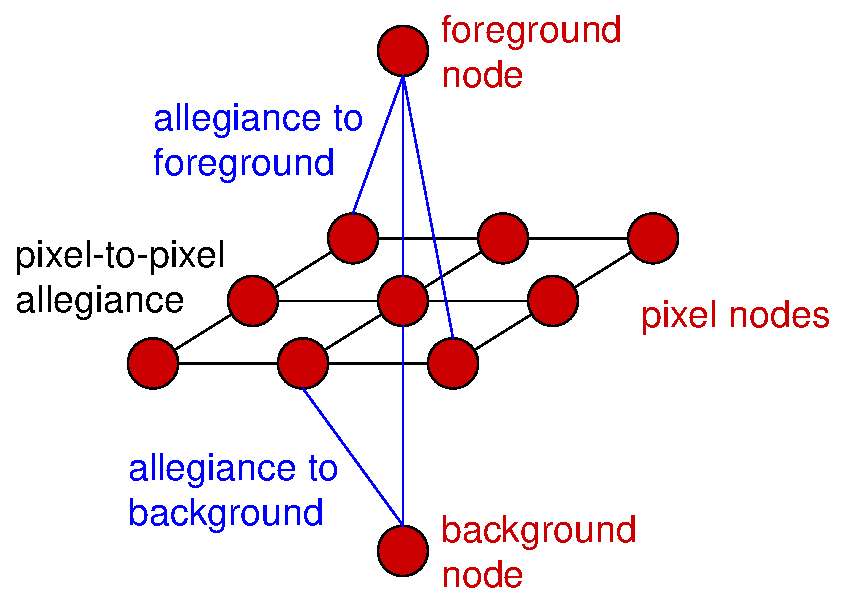
\includegraphics[width=7cm]{cut-graph1.eps}
\hspace{1cm}
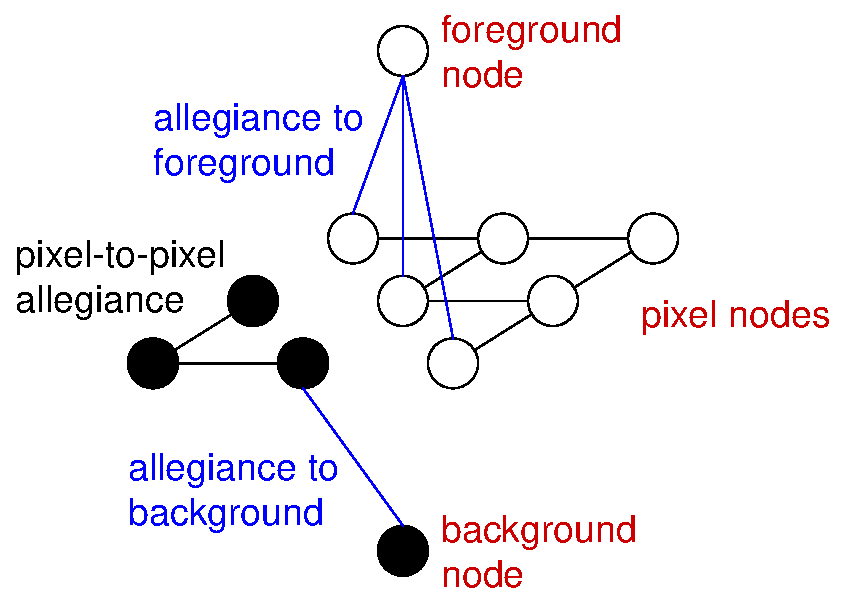
\includegraphics[width=7cm]{cut-graph2.eps}
\caption{ 
\label{fig:cut-graph}
%
A simple example of the graph cut algorithm in operation.  
The left graph represents the output of the point-of-contact 
processing.  Edges in the graphs are weighted by how much
it will cost to split connected nodes.  The bulk of the nodes
are in one-to-one correspondence with pixels in the image.
There are two extra nodes corresponding to the foreground and
background.  The goal is to split the graph into two by removing
edges.  The cost of the split is the sum of the weights on the 
edges removed.  There are good approximate algorithms for
finding a minimum cost solution [ref].
%
}
\end{center}
\end{figure*}

Use 16-connectivity (8 neighbors, plus cells connected by a
``knight'' move).

\fi


\begin{figure}[tbh]
  \centerline{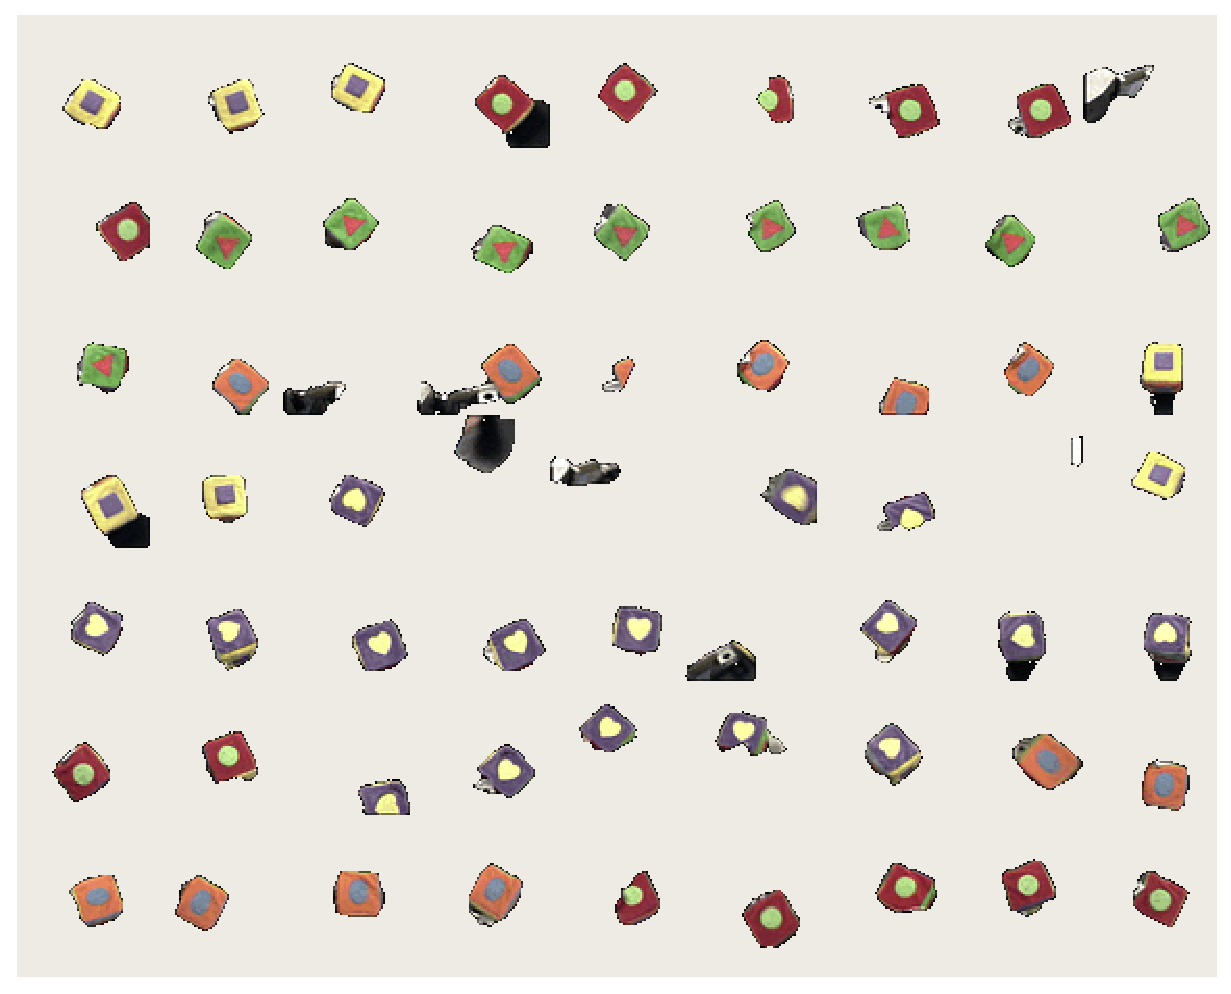
\includegraphics[width=9cm]{experiment-montage}}
  \caption{Sample results}
  \label{fig:sample-results}
\end{figure}

